\documentclass{article}
\usepackage{amsthm}
\usepackage{tikz}
\usepackage{amssymb}
\usetikzlibrary{automata, positioning, arrows}
\usetikzlibrary{calc}


\tikzset{
->, % makes the edges directed
>=stealth', % makes the arrow heads bold
node distance=3cm, % specifies the minimum distance between two nodes. Change if necessary.
every state/.style={thick, fill=gray!10}, % sets the properties for each ’state’ node
initial text=$ $, % sets the text that appears on the start arrow
}

\makeatletter
\def\lecture{\@ifnextchar[{\@lectureWith}{\@lectureWithout}}
\def\@lectureWith[#1]{\medbreak\refstepcounter{section}%
  \renewcommand{\leftmark}{Lecture \thesection}
  \noindent{\addcontentsline{toc}{section}{Lecture \thesection: #1\@addpunct{.}}%
  \sectionfont Lecture \thesection. #1\@addpunct{.}}\medbreak}
\def\@lectureWithout{\medbreak\refstepcounter{section}%
  \renewcommand{\leftmark}{Lecture \thesection}
  \noindent{\addcontentsline{toc}{section}{Lecture \thesection.}%
  \sectionfont Lecture \thesection.}\medbreak}
\makeatother

\makeatletter
\def\sectionfont{\normalfont}
\makeatother

\title{Teoria da computação}
\author{Rodrigo Santos}
\begin{document}
\maketitle


\theoremstyle{plain}
\newtheorem{xca}{Exercise}
\theoremstyle{definition}
\newtheorem{prob}{Problem}

\section{Problem set 3}

\begin{xca}
  Para cada uma das linguagens abaixo descreva um $AFD$ que a reconhece através do seu diagrama de estados e de uma definição formal
\end{xca}

\begin{prob}
  $L = \{0^{2n} \ | \ n \in \mathbb{N}\}$

  \begin{center}
    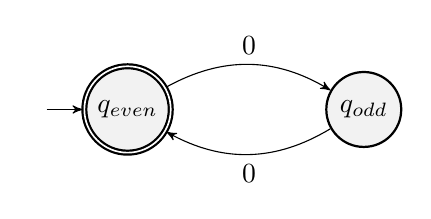
\begin{tikzpicture}
      \node[state, initial,accepting] (q1) {$q_{even}$};
      \node[state, right of=q1] (q2) {$q_{odd}$};
      \draw (q1) edge[bend left, above] node{0} (q2)
      (q2) edge[bend left, below] node{0} (q1);
    \end{tikzpicture}
  \end{center}

  A descrição formal do $AFD$ é:
  \begin{center}
    $M_1 = (\{q_{even},q_{odd}\}, \{0\},\delta,q_{even}, \{q_{even}\})$
  \end{center}
  onde $\delta$ é representado da seguinte maneira:
  \begin{table}[htbp]
    \centering
    \begin{tabular}{cclll}
      \multicolumn{1}{c|}{\textit{$\delta$}}   & \textit{0}                    & \textit{} & \textit{} & \textit{} \\ \cline{1-2}
      \multicolumn{1}{c|}{\textit{$q_{even}$}} & \textit{$q_{odd}$}            & \textit{} & \textit{} & \textit{} \\
      \multicolumn{1}{c|}{\textit{$q_{odd}$}}  & \textit{$q_{even}$}           & \textit{} & \textit{} & \textit{} \\
      \multicolumn{1}{l}{\textit{}}            & \multicolumn{1}{l}{\textit{}} & \textit{} & \textit{} & \textit{}
    \end{tabular}
  \end{table}
\end{prob}

\begin{prob}
  $L = \{(01)^n \ | \ n \in \mathbb{N}\}$

  \begin{center}
    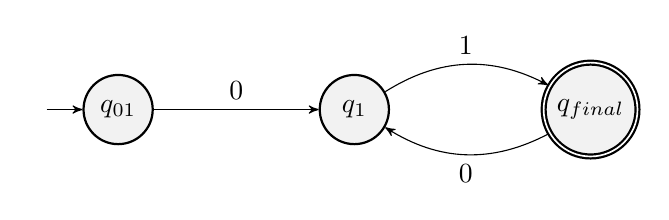
\begin{tikzpicture}
      \node[state, initial] (q1) {$q_{01}$};
      \node[state, right of=q1] (q2) {$q_{1}$};
      \node[state, accepting,right of=q2] (q3) {$q_{final}$};
      \draw (q1) edge[above] node{0} (q2)
      (q2) edge[bend left, above] node{1} (q3)
      (q3) edge[bend left, below] node{0} (q2);
    \end{tikzpicture}
  \end{center}
  \pagebreak
  A descrição formal do $AFD$ é:
  \begin{center}
    $M_2 = (\{q_{01},q_{1},q_{final}\}, \{0,1\},\delta,q_{01}, \{q_{final}\})$
  \end{center}
  onde $\delta$ é representado da seguinte maneira:
  \begin{table}[htbp]
    \centering
    \begin{tabular}{c|ccll}
      \textit{$\delta$}    & \textit{0}       & \textit{1}           & \textit{} & \textit{} \\ \cline{1-3}
      \textit{$q_{01}$}    & \textit{$q_{1}$} & \textit{$\perp$}     & \textit{} & \textit{} \\
      \textit{$q_{1}$}     & \textit{$\perp$} & \textit{$q_{final}$} & \textit{} & \textit{} \\
      \textit{$q_{final}$} & \textit{$q_1$}   & \textit{$\perp$}     & \textit{} & \textit{}
    \end{tabular}
  \end{table}
\end{prob}

\begin{prob}
  A linguagem $L$ das strings sobre $\{0, 1\}$ que contêm pelos menos dois $0's$ e pelo menos um $1$.

  \begin{center}
    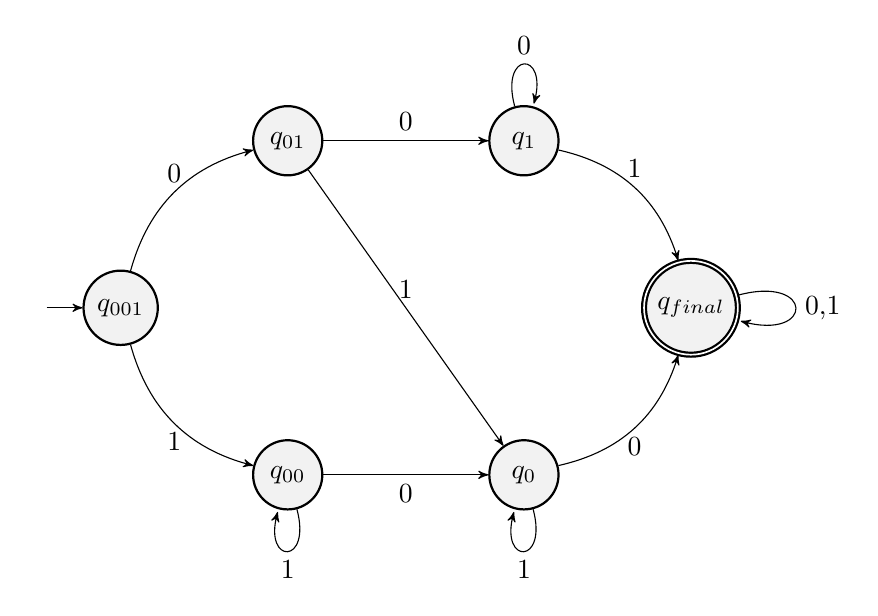
\begin{tikzpicture}
      \node[state, initial] (q001) {$q_{001}$};
      \node[state, above right of=q001] (q01) {$q_{01}$};
      \node[state, below right of=q001] (q00) {$q_{00}$};
      \node[state, right of=q01] (q1) {$q_{1}$};
      \node[state, right of=q00] (q0) {$q_{0}$};
      \node[state, accepting, below right of=q1] (qf) {$q_{final}$};
      \draw (q001) edge[bend left, above] node{0} (q01)
      (q001) edge[bend right, below] node{1} (q00)
      (q01) edge[above] node{0} (q1)
      (q01) edge[above] node{1} (q0)
      (q00) edge[below] node{0} (q0)
      (q00) edge[loop below] node{1} (q0)
      (q1) edge [bend left, above] node{1} (qf)
      (q1) edge [loop above] node{0} (q1)
      (q0) edge[bend right, below] node{0} (qf)
      (q0) edge[loop below] node{1} (q0)
      (qf) edge[loop right] node{0,1} (qf);
    \end{tikzpicture}
  \end{center}

  A descrição formal do $AFD$ é:
  \begin{center}
    $M_3 = (\{q_{001},q_{01},q_{00},q_{1}, q_{0},q_{final}\}, \{0,1\},\delta,q_{001}, \{q_{final}\})$
  \end{center}
  onde $\delta$ é representado da seguinte maneira:
  \begin{table}[htbp]
    \centering
    \begin{tabular}{c|cc}
      \textit{$\delta$}  & \textit{0}        & \textit{1}        \\ \hline
      \textit{$q_{001}$} & \textit{$q_{01}$} & \textit{$q_{00}$} \\
      \textit{$q_{00}$}  & \textit{$q_{0}$}  & \textit{$q_{00}$} \\
      \textit{$q_{01}$}  & \textit{$q_{1}$}  & \textit{$q_{0}$}  \\
      $q_{1}$            & $q_{1}$           & $q_{final}$       \\
      $q_{0}$            & $q_{final}$       & $q_{0}$           \\
      $q_{final}$        & $q_{final}$       & $q_{final}$
    \end{tabular}
  \end{table}
\end{prob}

\begin{prob}
  A linguagem $L$ das strings sobre $\{0, 1\}$ que contêm exatamente dois $0's$ e pelo menos dois $1's$.

  \begin{center}
    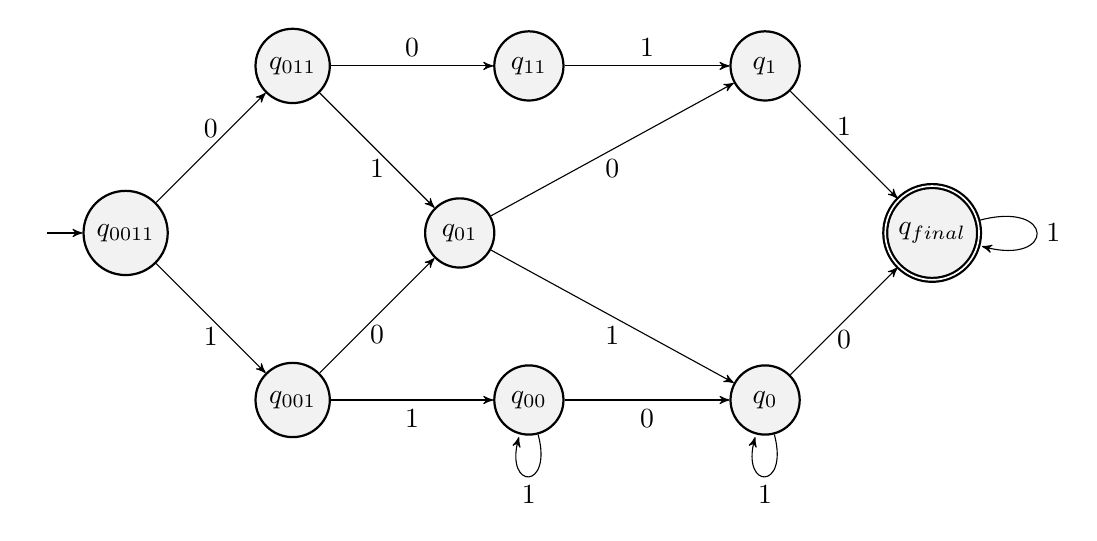
\begin{tikzpicture}
      \node[state, initial] (q0011) {$q_{0011}$};
      \node[state, above right of=q0011] (q011) {$q_{011}$};
      \node[state, below right of=q0011] (q001) {$q_{001}$};
      \node[state, right of=q011] (q11) {$q_{11}$};
      \node[state, below right of=q011] (q01) {$q_{01}$};
      \node[state, right of=q001] (q00) {$q_{00}$};
      \node[state, right of=q00] (q0) {$q_{0}$};
      \node[state, right of=q11] (q1) {$q_{1}$};
      \node[state, below right of=q1, accepting] (qf) {$q_{final}$};
      \draw (q0011) edge[above] node{0} (q011)
      (q0011) edge[below] node{1} (q001)
      (q011) edge[below] node{1} (q01)
      (q011) edge[above] node{0} (q11)
      (q001) edge[below] node{1} (q00)
      (q001) edge[below] node{0} (q01)
      (q01) edge[below] node{0} (q1)
      (q01) edge[below] node{1} (q0)
      (q11) edge[above] node{1} (q1)
      (q00) edge[below] node{0} (q0)
      (q00) edge[loop below] node{1} (q00)
      (q0) edge[loop below] node{1} (q0)
      (q0) edge[below] node{0} (qf)
      (q1) edge[above] node{1} (qf)
      (qf) edge[loop right] node{1} (qf);
    \end{tikzpicture}
  \end{center}

  A descrição formal do $AFD$ é:
  \begin{center}
    $M_4 = (\{q_{0011},q_{011},q_{001},q_{11},q_{01},q_{00},q_{1}, q_{0},q_{final}\}, \{0,1\},\delta,q_{0011}, \{q_{final}\})$
  \end{center}
  onde $\delta$ é representado da seguinte maneira:

  \begin{table}[htbp]
    \centering
    \begin{tabular}{c|cc}
      \textit{$\delta$}   & \textit{0}         & \textit{1}         \\ \hline
      \textit{$q_{0011}$} & \textit{$q_{011}$} & \textit{$q_{001}$} \\
      \textit{$q_{001}$}  & \textit{$q_{01}$}  & \textit{$q_{00}$}  \\
      \textit{$q_{011}$}  & \textit{$q_{11}$}  & \textit{$q_{01}$}  \\
      $q_{01}$            & $q_{0}$            & $q_{1}$            \\
      $q_{00}$            & $q_{0}$            & $q_{00}$           \\
      $q_{11}$            & $\perp$            & $q_{1}$            \\
      $q_{0}$             & $q_{final}$        & $q_{0}$            \\
      $q_{1}$             & $\perp$            & $q_{final}$        \\
      $q_{final}$         & $\perp$            & $q_{final}$
    \end{tabular}
  \end{table}
\end{prob}

\pagebreak

\begin{prob}
  A linguagem $L$ das strings sobre $\{0, 1\}$ com um número par de $0's$ e um número ímpar de $1's$.

  \begin{center}
    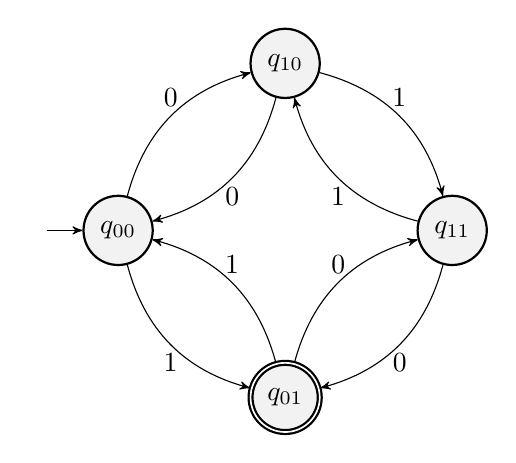
\begin{tikzpicture}
      \node[state, initial] (q00) {$q_{00}$};
      \node[state, above right of=q00] (q10) {$q_{10}$};
      \node[state, below right of=q00, accepting] (q01) {$q_{01}$};
      \node[state, above right of=q01] (q11) {$q_{11}$};
      \draw (q00) edge[bend left, above] node{0} (q10)
      (q00) edge[bend right, below] node{1} (q01)
      (q10) edge[bend left, below] node{0} (q00)
      (q10) edge[bend left, above] node{1} (q11)
      (q01) edge[bend right, above] node{1} (q00)
      (q01) edge[bend left, above] node{0} (q11)
      (q11) edge[bend left, below] node{0} (q01)
      (q11) edge[bend left, below] node{1} (q10);
    \end{tikzpicture}
  \end{center}

  A descrição formal do $AFD$ é:
  \begin{center}
    $M_5 = (\{q_{00},q_{10},q_{01},q_{11}\}, \{0,1\},\delta,q_{00}, \{q_{01}\})$
  \end{center}
  onde $\delta$ é representado da seguinte maneira:
  \begin{table}[htbp]
    \centering
    \begin{tabular}{c|cc}
      \textit{$\delta$} & \textit{0}        & \textit{1}        \\ \hline
      \textit{$q_{00}$} & \textit{$q_{10}$} & \textit{$q_{01}$} \\
      \textit{$q_{10}$} & \textit{$q_{00}$} & \textit{$q_{11}$} \\
      \textit{$q_{01}$} & \textit{$q_{11}$} & \textit{$q_{00}$} \\
      $q_{11}$          & $q_{01}$          & $q_{10}$
    \end{tabular}
  \end{table}
\end{prob}

\begin{prob}
  A linguagem $L$ das strings sobre $\{0, 1\}$ que não contêm a substring $010$.

  \begin{center}
    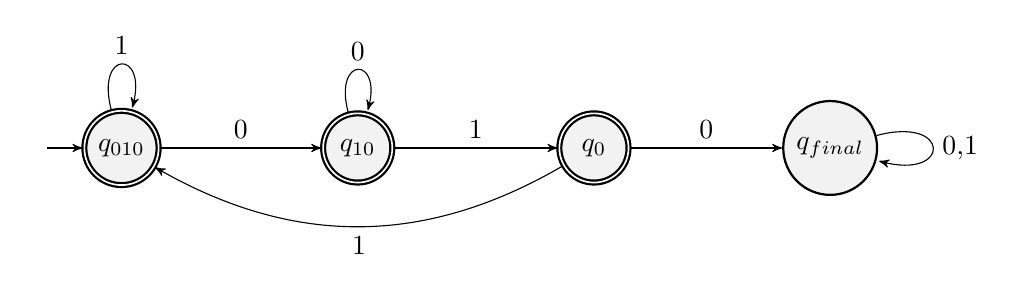
\begin{tikzpicture}
      \node[state, initial, accepting] (q010) {$q_{010}$};
      \node[state, accepting, right of=q010] (q10) {$q_{10}$};
      \node[state, accepting, right of=q10] (q0) {$q_{0}$};
      \node[state, right of=q0] (qf) {$q_{final}$};
      \draw (q010) edge[loop above] node{1} (q010)
      (q010) edge[above] node{0} (q10)
      (q10) edge[loop above] node{0} (q10)
      (q10) edge[above] node{1} (q0)
      (q0) edge[above] node{0} (qf)
      (q0) edge[bend left, below] node{1} (q010)
      (qf) edge[loop right] node{0,1} (qf);
    \end{tikzpicture}
  \end{center}

  A descrição formal do $AFD$ é:
  \begin{center}
    $M_6 = (\{q_{010},q_{10},q_{0},q_{final}\}, \{0,1\},\delta,q_{010}, \{q_{010},q_{10},q_{0}\})$
  \end{center}
  \pagebreak
  onde $\delta$ é representado da seguinte maneira:

  \begin{table}[htbp]
    \centering
    \begin{tabular}{c|cc}
      \textit{$\delta$}  & \textit{0}           & \textit{1}         \\ \hline
      \textit{$q_{010}$} & \textit{$q_{10}$}    & \textit{$q_{010}$} \\
      \textit{$q_{10}$}  & \textit{$q_{10}$}    & \textit{$q_{0}$}   \\
      \textit{$q_{0}$}   & \textit{$q_{final}$} & \textit{$q_{010}$} \\
      $q_{final}$        & $q_{final}$          & $q_{final}$
    \end{tabular}
  \end{table}
\end{prob}

\begin{prob}
  A linguagem $L$ das strings sobre $\{0, 1\}$ com um número par de $0's$ e em que cada $0$ é sempre seguido de pelo menos um $1$.

  \begin{center}
    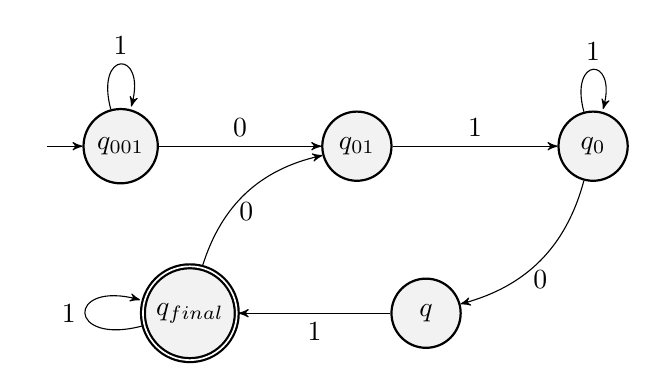
\begin{tikzpicture}
      \node[state, initial] (q001) {$q_{001}$};
      \node[state, right of=q001] (q01) {$q_{01}$};
      \node[state, right of=q01] (q0) {$q_{0}$};
      \node[state, below left of=q0] (q) {$q$};
      \node[state, accepting,left of=q] (qf) {$q_{final}$};
      \draw (q001) edge[loop above] node{1} (q001)
      (q001) edge[above] node{0} (q01)
      (q01) edge[above] node{1} (q0)
      (q0) edge[loop above] node{1} (q0)
      (q0) edge[bend left, below] node{0} (q)
      (q) edge[below] node{1} (qf)
      (qf) edge[bend left, below] node{0} (q01)
      (qf) edge[loop left] node{1} (qf);
    \end{tikzpicture}
  \end{center}

  A descrição formal do $AFD$ é:
  \begin{center}
    $M_7 = (\{q_{001},q_{01},q_{0},q,q_{final}\}, \{0,1\},\delta,q_{001}, \{q_{final}\})$
  \end{center}
  onde $\delta$ é representado da seguinte maneira:

  \begin{table}[htbp]
    \centering
    \begin{tabular}{c|cc}
      \textit{$\delta$}  & \textit{0}        & \textit{1}         \\ \hline
      \textit{$q_{001}$} & \textit{$q_{01}$} & \textit{$q_{001}$} \\
      \textit{$q_{01}$}  & \textit{$\perp$}  & \textit{$q_{0}$}   \\
      \textit{$q_{0}$}   & \textit{$q$}      & \textit{$q_{0}$}   \\
      $q$                & $\perp$           & $q_{final}$        \\
      $q_{final}$        & $q_{01}$          & $q_{final}$
    \end{tabular}
  \end{table}
\end{prob}

\begin{prob}
  A linguagem L das strings sobre $\{0\}$ com tamanho divisível por $2$ ou por $3$. $q_{ij}$ onde $i = n \% 2$ e $j = n \% 3$.

  \begin{center}
    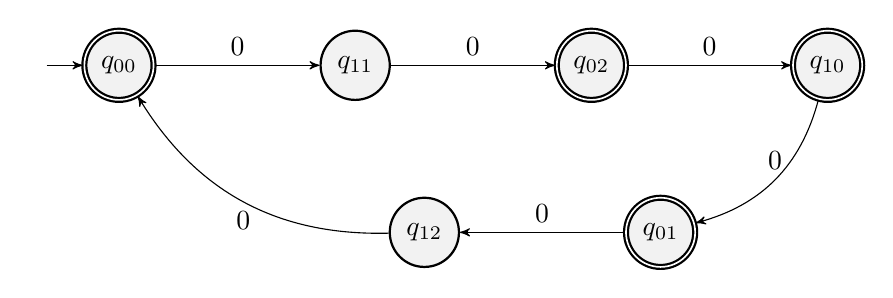
\begin{tikzpicture}
      \node[state, accepting, initial] (q00) {$q_{00}$};
      \node[state, right of=q00] (q11) {$q_{11}$};
      \node[state, accepting, right of=q11] (q02) {$q_{02}$};
      \node[state, accepting, right of=q02] (q10) {$q_{10}$};
      \node[state, accepting, below left of=q10] (q01) {$q_{01}$};
      \node[state, left of=q01] (q12) {$q_{12}$};
      \draw (q00) edge[above] node{0} (q11)
      (q11) edge[above] node{0} (q02)
      (q02) edge[above] node{0} (q10)
      (q10) edge[bend left, above] node{0} (q01)
      (q01) edge[above] node{0} (q12)
      (q12) edge[bend left, below] node{0} (q00);
    \end{tikzpicture}
  \end{center}

  A descrição formal do $AFD$ é:
  \begin{center}
    $M_8 = (\{q_{00},q_{11},q_{02},q_{10},q_{01},q_{12}\}, \{0\},\delta,q_{00}, \{q_{00},q_{02},q_{10},q_{01}\})$
  \end{center}
  onde $\delta$ é representado da seguinte maneira:
  \begin{table}[htbp]
    \centering
    \begin{tabular}{c|c}
      \textit{$\delta$} & \textit{0}        \\ \hline
      \textit{$q_{00}$} & \textit{$q_{11}$} \\
      \textit{$q_{11}$} & \textit{$q_{02}$} \\
      \textit{$q_{02}$} & \textit{$q_{10}$} \\
      $q_{10}$          & $q_{01}$          \\
      $q_{01}$          & $q_{12}$          \\
      $q_{12}$          & $q_{00}$
    \end{tabular}
  \end{table}
\end{prob}

\begin{prob}
  A linguagem $L$ das strings sobre $\{A, C, G, T \}$ que contêm pelo menos uma ocorrência da substring $ACT$.

  \begin{center}
    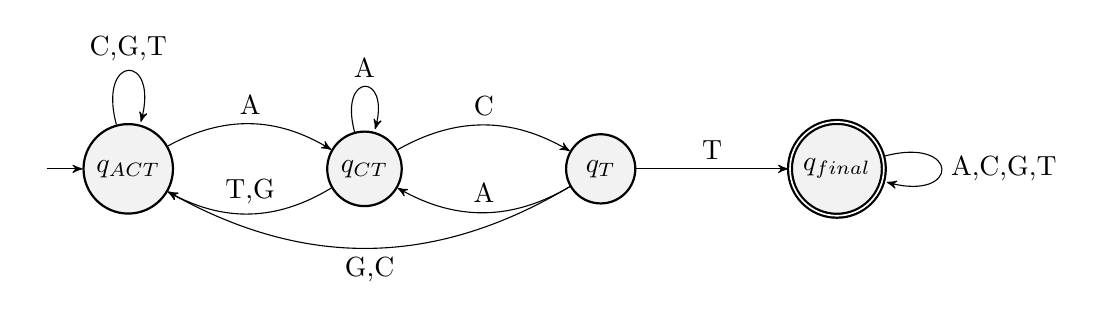
\begin{tikzpicture}
      \node[state, initial] (q0) {$q_{ACT}$};
      \node[state, right of=q0] (q1) {$q_{CT}$};
      \node[state, right of=q1] (q2) {$q_{T}$};
      \node[state, right of=q2, accepting] (qf) {$q_{final}$};
      \draw (q0) edge[loop above] node{C,G,T} (q0)
      (q0) edge[bend left, above] node{A} (q1)
      (q1) edge[loop above] node{A} (q1)
      (q1) edge[bend left, above] node{T,G} (q0)
      (q1) edge[bend left, above] node{C} (q2)
      (q2) edge[bend left, above] node{A} (q1)
      (q2) edge[above] node{T} (qf)
      (qf) edge[loop right] node{A,C,G,T} (qf)
      (q2) edge[bend left, below] node{G,C} (q0);
    \end{tikzpicture}
  \end{center}

  A descrição formal do $AFD$ é:
  \begin{center}
    $M_9 = (\{q_{ACT},q_{CT},q_{T},q_{final}\}, \{A,C,G,T\},\delta,q_{ACT}, \{q_{final}\})$
  \end{center}
  onde $\delta$ é representado da seguinte maneira:

  \begin{table}[htbp]
    \centering
    \begin{tabular}{c|cccc}
      \textit{$\delta$} & \textit{A}  & C           & G           & T           \\ \hline
      $q_{ACT}$         & $q_{CT}$    & $q_{ACT}$   & $q_{ACT}$   & $q_{ACT}$   \\
      $q_{CT}$          & $q_{CT}$    & $q_{T}$     & $q_{ACT}$   & $q_{ACT}$   \\
      $q_{T}$           & $q_{CT}$    & $q_{ACT}$   & $q_{ACT}$   & $q_{final}$ \\
      $q_{final}$       & $q_{final}$ & $q_{final}$ & $q_{final}$ & $q_{final}$
    \end{tabular}
  \end{table}
\end{prob}

\pagebreak

\begin{prob}
  $L = \varnothing $ sobre $\{0,1\}$

  \begin{center}
    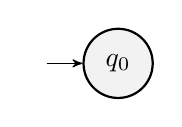
\begin{tikzpicture}
      \node[state, initial] (q0) {$q_0$};
    \end{tikzpicture}
  \end{center}

  A descrição formal do $AFD$ é:
  \begin{center}
    $M_{10} = (\{q_{0}\}, \{0,1\},\delta,q_{0}, \varnothing)$
  \end{center}
  onde $\delta$ é representado da seguinte maneira: $\delta:S\times \Sigma\to S$ dada por $\delta(q_0,0)=\bot$ e $\delta(q_0,1)=\bot$
\end{prob}

\begin{prob}
  $L = {\varepsilon}$ sobre $\{0,1\}$

  \begin{center}
    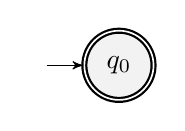
\begin{tikzpicture}
      \node[state, initial, accepting] (q0) {$q_0$};
    \end{tikzpicture}
  \end{center}

  A descrição formal do $AFD$ é:
  \begin{center}
    $M_{11} = (\{q_{0}\}, \{0,1\},\delta, q_{0}, \{q_0\})$
  \end{center}
  onde $\delta$ é representado da seguinte maneira: $\delta:S\times \Sigma\to S$ dada por $\delta(q_0,0)=\bot$ e $\delta(q_0,1)=\bot$
\end{prob}

\begin{prob}
  $L = \{0, 1\}^{*} \setminus \{\varepsilon\}$

  \begin{center}
    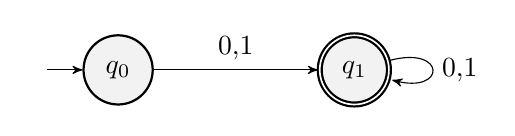
\begin{tikzpicture}
      \node[state, initial] (q0) {$q_{0}$};
      \node[state, right of=q0, accepting] (q1) {$q_{1}$};
      \draw (q0) edge[above] node{0,1} (q1)
      (q1) edge[loop right] node{0,1} (q1);
    \end{tikzpicture}
  \end{center}

  A descrição formal do $AFD$ é:
  \begin{center}
    $M_{12} = (\{q_{0},q_1\}, \{0,1\},\delta, q_{0}, \{q_1\})$
  \end{center}
  onde $\delta$ é representado da seguinte maneira:
  \begin{table}[htbp]
    \centering
    \begin{tabular}{c|cc}
      \textit{$\delta$} & \textit{0} & 1       \\ \hline
      $q_{0}$           & $q_{1}$    & $q_{1}$ \\
      $q_{1}$           & $q_{1}$    & $q_{1}$
    \end{tabular}
  \end{table}
\end{prob}

\end{document}